\documentclass ../main.tex]{subfiles}

\begin{document}



\vspace{3cm}
\chapter{Nociones Previas}

En el estudio de partículas elementales, notamos que experimentalmente se observan efectos tanto cuanticos como relativistas fenomenologicamente. Por lo que para trabajar con ellas se deberá tener en cuenta tanto la mécanica cuántica como la relatividad especial. La teoría con la que más nos acomodará trabajar será la \textbf{Teoría Cuantica de Campos (QFT)} pues tomará ambos efectos en consideración y nos permitirá estudiar eventos que sucedan a velocidades comparables con la velocidad de la luz $c$ en regiones pequeñas.\\

\begin{figure}[h] % "h" intenta colocar la imagen aquí
    \centering
    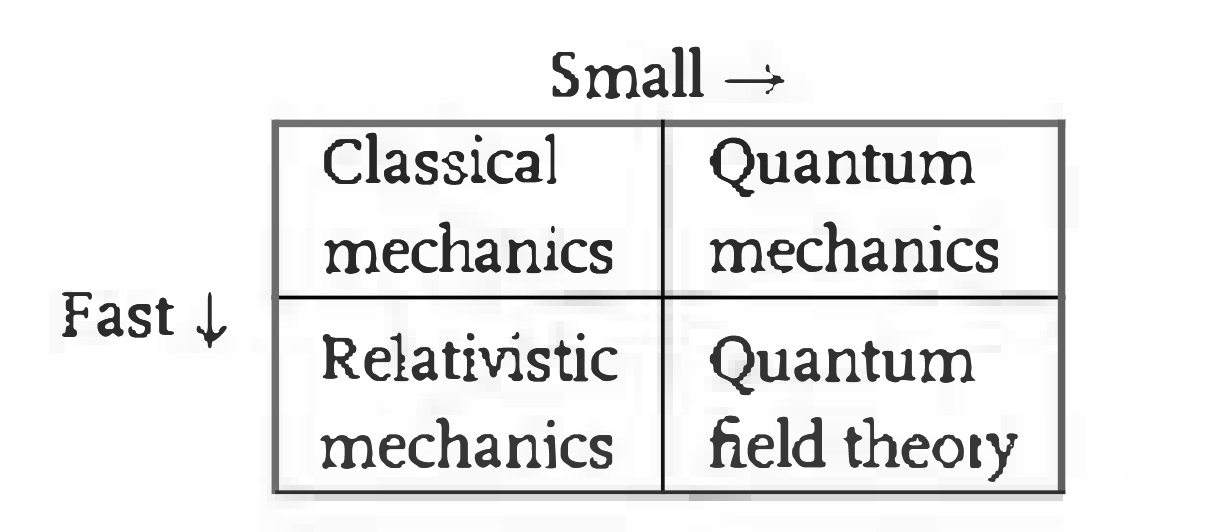
\includegraphics[width=0.5\textwidth]{img/Captura de pantalla 2025-03-29 000744.png}
    \label{fig:graf_QFT}
\end{figure}


Es por esto que para poder estudiar QFT se deberán tener nociones tanto de mécanica clásica como cuántica. En este apunte, no se considerarán los efectos del campo gravitacional. Como las interacciones a estudiar ocurren en regiones pequeñas, el efecto gravitacional será considerado despreciable. 

%quizas podríamos poner aca el decaimiento beta o otros ejemplos pero no sabia cuales poner pq no todos son d clasica 

\section{Primera clase}

\subsection{Derivación de las Ecuaciones de Euler-Lagrange}

Sea la acción $S[q(t)]$, donde $q(t)$ son las coordenadas generalizadas del sistema. 

\begin{equation}
    S[q(t)] = \int dt L(q, \dot{q})
\end{equation}

Ahora, ¿Cómo cambia $S$ si $q(t)$ cambia un poco?\\

Sea $q(t)$ una función dependiente del tiempo, bien definida en el intervalo $t \in [t_1 , t_2]$. Donde los puntos $q(t_1)$ y $q(t_2)$ estarán fijos, de manera que aunque $q(t)$ cambie su valor en $t_1$ y $t_2$ no cambiara. Así, como se muestra en la figura [\textbf{citar}], si consideramos todos los caminos que puede tomar $q(t)$, diferenciados por una diferencia infinitesimal $\delta q = \Phi(t)$ que a su vez será dependiente del tiempo, se podrá variar la acción. 


[foto clasica de la invarianza d la acción]


\begin{align}
    \delta S &= S[q(t) + \phi(t)] - S[q(t)] \notag \\
    &= \int_{t_1}^{t_2}dt L(q(t) + \phi(t), \frac{d}{dt}\left(q + \Phi \right)) -\int_{t_1}^{t_2}dt L(q(t), \dot{q}(t)) \label{eq:var-accion1}\\
\end{align}

Además, considerando que: 

\begin{equation}
    f(x +\epsilon_1, y + \epsilon_2) = f(x,y) + \frac{\partial f}{\partial x}\epsilon_1 + \frac{\partial f}{\partial y}\epsilon_2 + \mathcal{O}(\epsilon_1^2, \epsilon_2^2, \epsilon_1, \epsilon_2) \label{eq:ec_1}
\end{equation}

Por lo tanto, introduciendo \ref{eq:ec_1} con $f(x +\epsilon_1, y + \epsilon_2) = L(q(t) + \phi(t), \frac{d}{dt}\left(q + \Phi \right))$ en \ref{eq:var-accion1}.

\begin{align*}
    \delta S &=  \int_{t_1}^{t_2}dt \left( L(q(t),\dot{q}(t)) + \frac{\partial L}{\partial q}\Phi + \frac{\partial L}{\partial \dot{q}} \frac{d\Phi}{dt} \right) -  \int_{t_1}^{t_2}dt L(q(t), \dot{q}(t))\\ 
    &=  \int_{t_1}^{t_2}dt  \left(\frac{\partial L}{\partial q}\Phi + \frac{\partial L}{\partial \dot{q}} \frac{d\Phi}{dt} \right) \\
    &=  \int_{t_1}^{t_2}dt  \left(\frac{\partial L}{\partial q}\Phi + \frac{d}{dt}\left( \Phi \frac{\partial L}{\partial \dot{q}} \right) - \frac{d}{dt}\left( \frac{\partial L}{\partial \dot{q}} \right)\Phi \right) \\
    &=  \int_{t_1}^{t_2}dt \frac{d}{dt}\left( \Phi \frac{\partial L}{\partial \dot{q}} \right) + \int_{t_1}^{t_2}dt \Phi \left(\frac{\partial L}{\partial q}- \frac{d}{dt}\left( \frac{\partial L}{\partial \dot{q}} \right) \right) \\
    &= 0 + + \int_{t_1}^{t_2}dt \Phi \left(\frac{\partial L}{\partial q}- \frac{d}{dt}\left( \frac{\partial L}{\partial \dot{q}} \right) \right) \\
    \delta S &=\int_{t_1}^{t_2}dt \Phi \left(\frac{\partial L}{\partial q}- \frac{d}{dt}\left( \frac{\partial L}{\partial \dot{q}} \right) \right).\\
\end{align*}

Si se asume que el princiío de acción es estacionario $\delta S = 0$. Entonces: 

\begin{equation}
    \int_{t_1}^{t_2}dt \Phi \left(\frac{\partial L}{\partial q}- \frac{d}{dt}\left( \frac{\partial L}{\partial \dot{q}} \right) \right) = 0 \label{eq:var-accion2}
\end{equation}

Finalmente, considerando a $f(t)$ arbitraria, en \ref{eq:var-accion2} el integrando de la integral deberá ser igual a cero. Por lo tanto, 

\begin{equation}
    \frac{\partial L}{\partial q} - \frac{d}{dt} \left( \frac{\partial L}{\partial \dot{q}} \right) = 0
\end{equation}












\end{document}
